\title{Das kleine Segel 1x1}
%\author{
%}
\date{\today}

\documentclass[12pt]{article}
\usepackage[utf8]{inputenc}

\usepackage{stmaryrd}
\usepackage{graphicx}
\usepackage{hyperref}

\begin{document}
\maketitle

\begin{abstract}
Dieser Text soll eine kurze Einführung in das Thema Segeln sein. Es ist dafür gedacht um im Segeln Unerfahren die Grundbegriffe näher zu bringen, um mit einen erfahrenen Skipper eine längere Tour durchführen zu können.
\end{abstract}

\section{Begriffe}
Dies sind die wichtigen Begriffe, die alle Mitsegler kennen sollten, damit der Skipper präzise Anweisungen geben kann. Dies erhöht die Sicherheit und vermeidet Chaos.

\paragraph{Windrichtung}
Die Windrichtung ist für jeden leicht ersichtlich. Was nicht intuitiv zu verstehen ist, wie die Windrichtung angegeben wird. Die Windrichtung ist die Himmelsrichtung aus der der Wind kommt.

\paragraph{Bug}
Der vordere Teil des Bootes. Dies bezieht sich auf die Fahrtrichtung also der Teil des Bootes der spitz zuläuft.

\paragraph{Heck}
Der hintere Teil des Bootes. Also die Gegenseite vom Bug.

\paragraph{Backbord}
In Fahrtrichtung gesehen die linke Seite des Bootes. Den Seiten den Bootes werden auch Farben zugewiesen, damit man an Hand von Signallampen nachts die Fahrtrichtung erkennen kann. Die zugewiesene Farbe für Backbord ist \textbf{rot}.

\paragraph{Steuerbord}
In Fahrtrichtung gesehen die rechte Seite des Bootes. Die zugewiesene Farbe für Steuerbord ist \textbf{grün}.

\paragraph{Kurs}
Ein Kurs kann auf einen Segelboot zwei Bedeutungen haben. Zum einen bezeichnet es den Kurs den das Schiff relativ zum Magnetfeld macht. Also die Richtung in Grad, die man auf einem Kompass ablesen.

Zusätzlich kann ein Kurs den Kurs zum Wind bezeichnen. Die Kurse unterscheidet man nach dem Winkel zwischen der Windrichtung und dem Kurs des Bootes.

\paragraph{Tampen}
Seil

\paragraph{Schot}
Damit das Boot optimal voran kommt, muss das Segel passend zum Kurs zum Wind eingestellt werden.

Dies geschieht über Schoten - Tampen, die an den Segeln befestigt sind. Jedes Segel hat eigene Schoten. Eine Übersicht über alle Schoten findet ihr in Bild \ref{schoten}.

\begin{figure}[h!]
\begin{center}
\label{schoten}
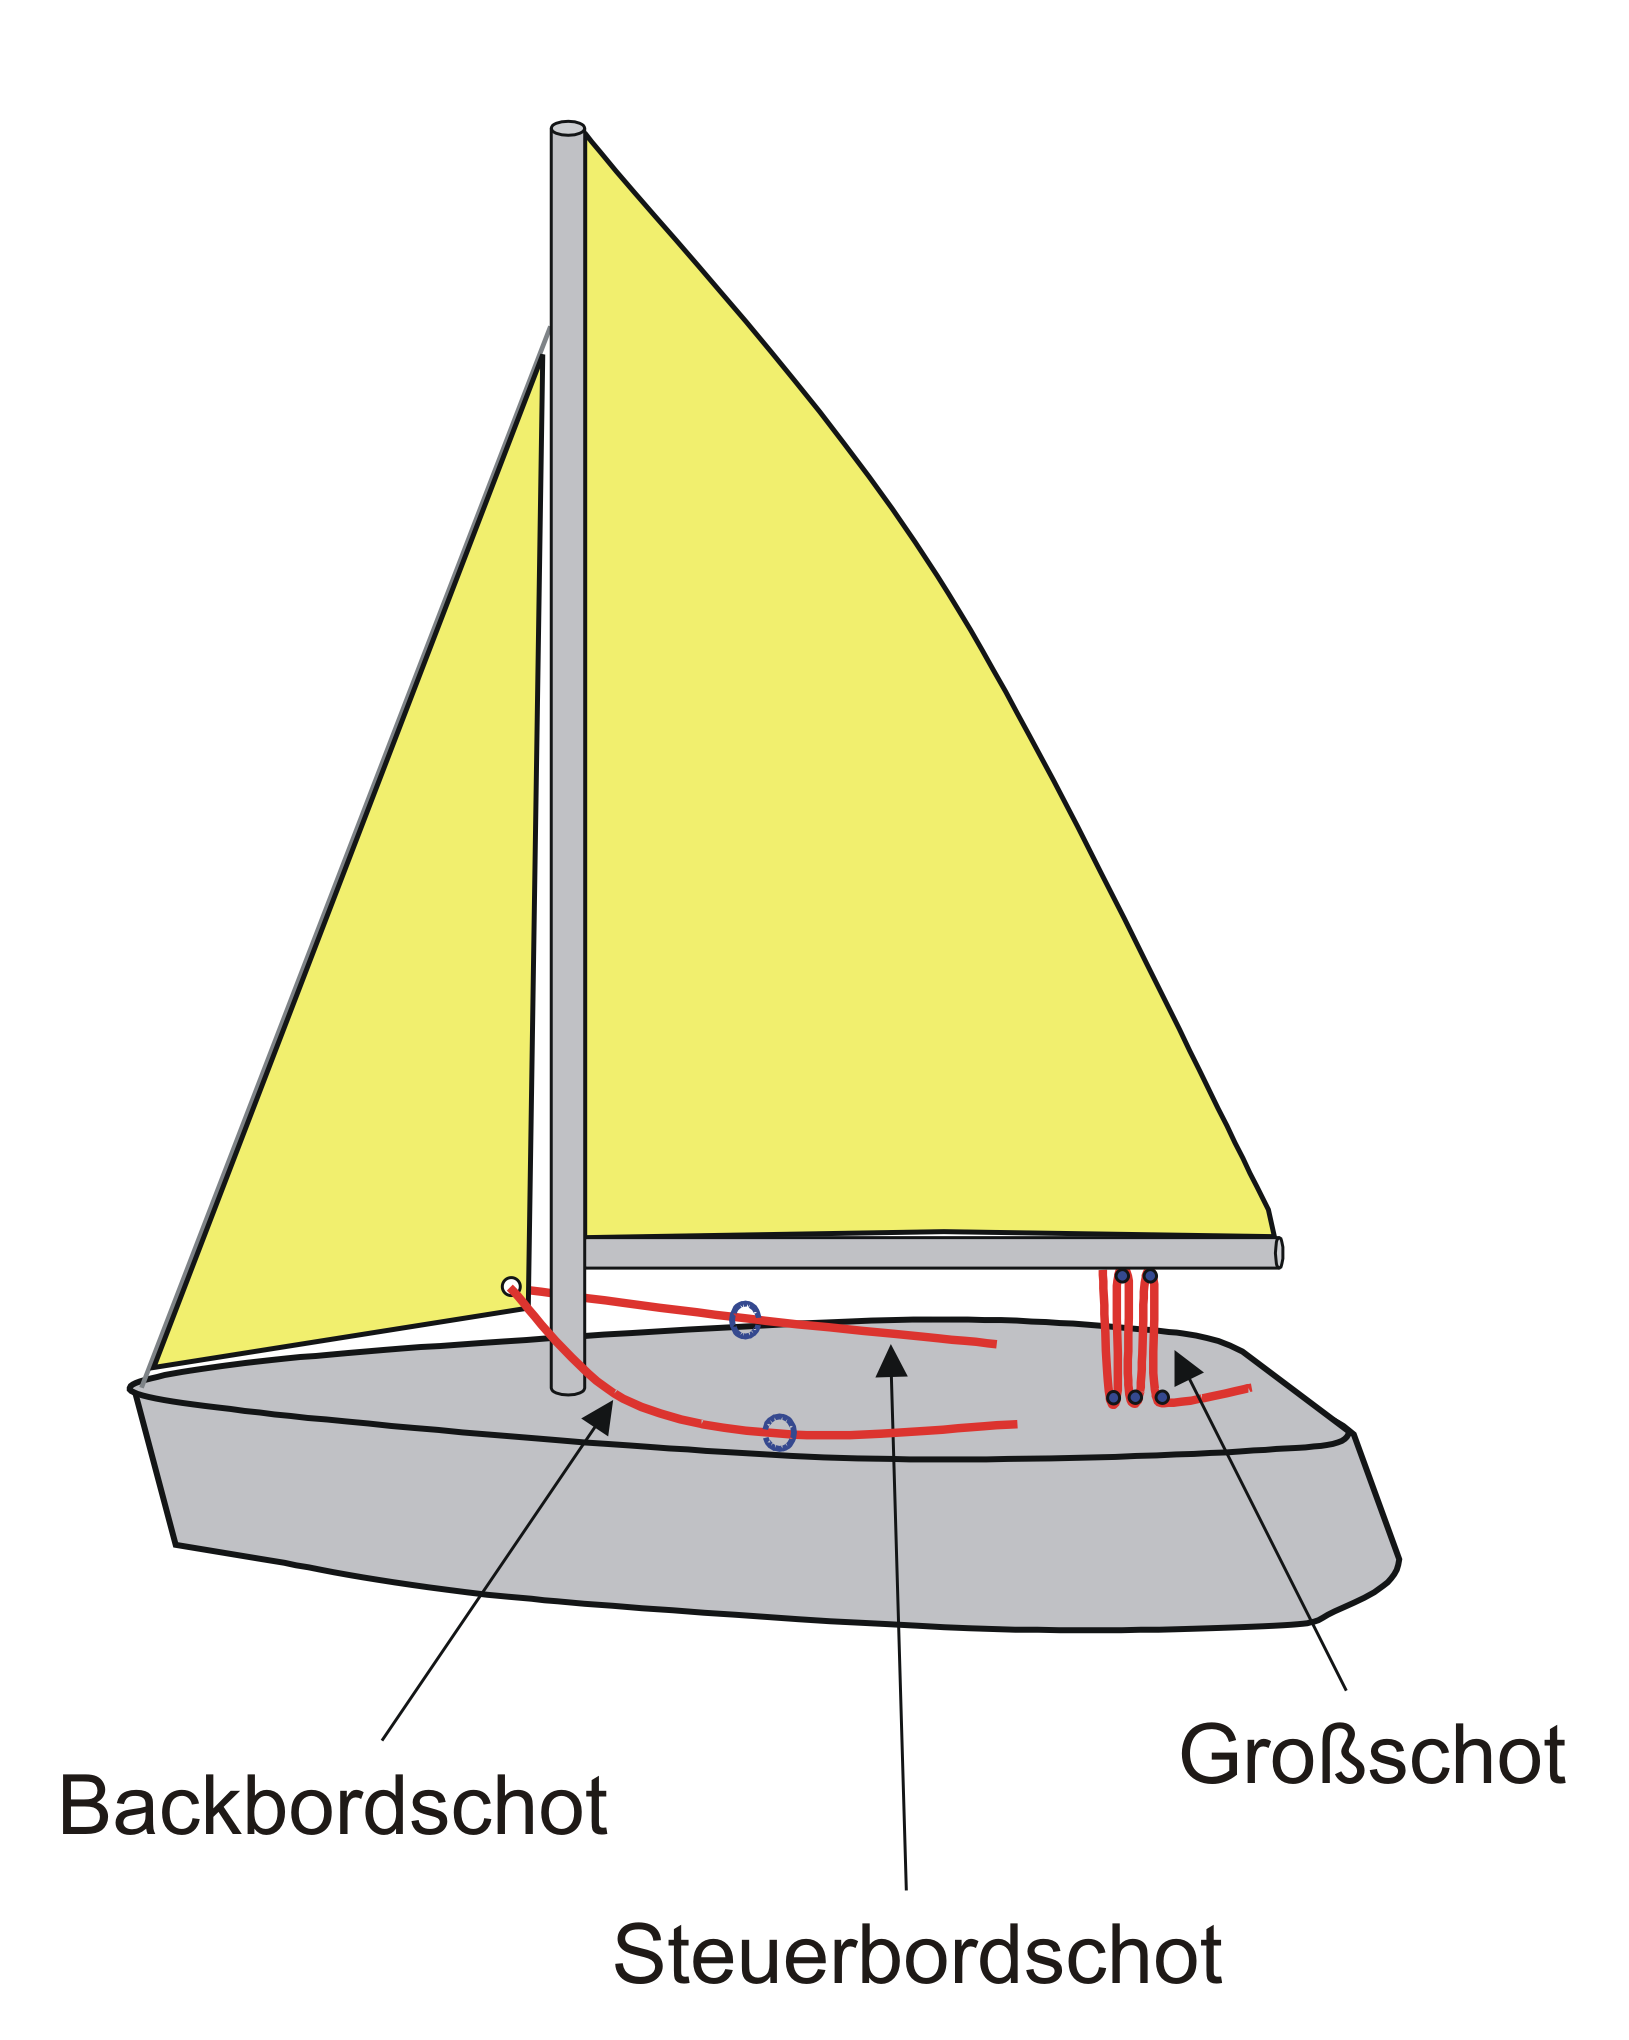
\includegraphics[scale=0.4]{bilder/schoten.png}
\end{center}
\caption{Die Schot einer Yacht}
\end{figure}

\paragraph{Fallen}
Um die Segel aufzuspannen sind sie oben an der Mastspitze befestigt. Diese Befestigungen werden mit Tampen realisiert, die von oben am Mast entlang geführt. Diese Tampen werden Fallen genannt.

\paragraph{Wanten und Stagen (Stehendes Gut)}
Der Mast wird mit Stahlseilen am Boot verspannt. Würde man dies nicht tun, würde der Mast beim Segeln unter der Belastung abbrechen.

Die Stagen spannen den Mast nach Vorne und Hinten ab, die Wanten zu den Seiten. Beide sind in Bild \ref{segel} eingezeichnet.

\paragraph{Wende und Halse}
bezeichnen Änderungen des Kurses zum Wind bei denen sich die Seite auf der die Segel gefahren werden ändern.

\section{Segel}

\begin{figure}[h!]
\begin{center}
\label{segel}
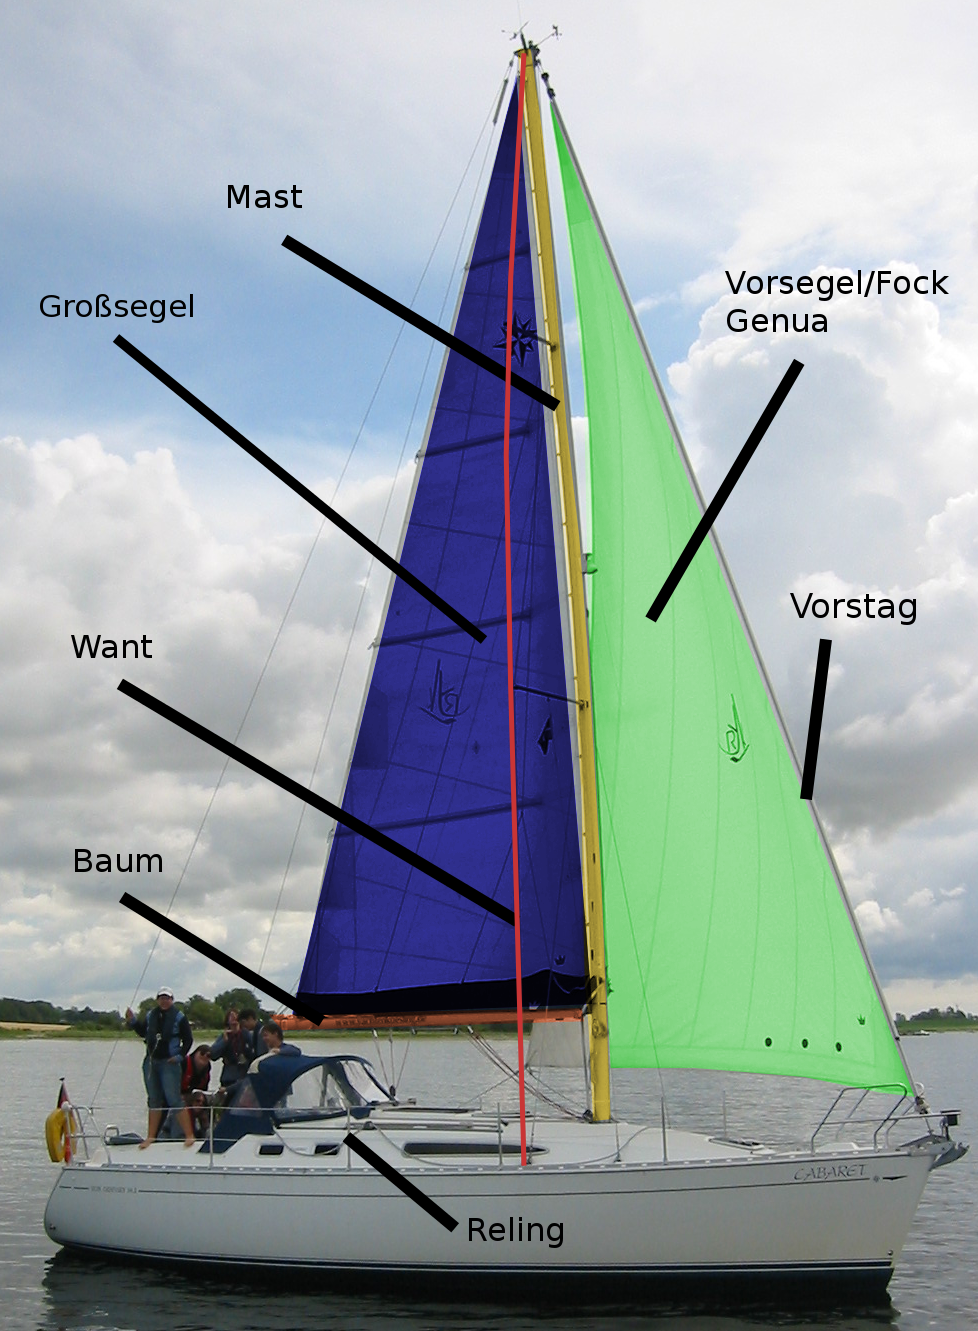
\includegraphics[scale=0.2]{bilder/yacht.png}
\end{center}
\caption{Die Segel einer Yacht}
\end{figure}

Eine moderne Segelyacht hat zwei Segel. Ein Großsegel und ein Vorsegel.
Das Vorsegel wird je nach Größe auch Fock oder Genua bezeichnet.

Das Großsegel wird hinter dem Mast gefahren und hat einen Baum am unteren Ende.

\section{Packliste}
Dies ist eine Liste der Sachen an die man unbedingt denken muss. Sie ist nur eine Referenz und erhebt keinen Anspruch auf Vollständigkeit. Als Transportmittel nutzt ihr bitte eine flexible Tasche/Rucksack/Seesack. Hartschalenkoffer lassen sich schlecht verstauen.

\subsection*{Was ist schon da?}
\begin{itemize}
\renewcommand{\labelitemi}{$\boxempty$}
\item Schwimmweste
\item Geschirr und Besteck
\item Matratze
\end{itemize}

\subsection*{Was muss?}
\begin{itemize}
\renewcommand{\labelitemi}{$\boxempty$}
\item Schlafsack
\item Bettlacken
\item Kissen
\item Brillenband
\item Waschsachen
\item Badesachen
\item Regenjacke(am besten eine feste) mit Kaputze oder Südwester
\item Regenhose
\item Gummistiefel
\item Schuhe mit abriebfreier Sohle
\item Genug warme Sachen (eine Mütze ist vielleicht auch angebracht)
\item und was man sonst noch alles zum Campen mitnehmen würde
\end{itemize}

\subsection*{Was kann?}
\begin{itemize}
\renewcommand{\labelitemi}{$\boxempty$}
\item Segelhandschuhe

\end{itemize}

Eine zusätzliche Inspiration kann diese Liste sein: \href{http://www.pc-ostsee.de/yachtcharter/sites/download/Packliste.pdf}{Packliste PCO}

\include{anfahrt} %Anfahrt Beschreibung

\end{document}
